\documentclass[a4paper, 12pt, oneside, titlepage]{article} %{\parskip}
\usepackage[top=2.54cm, bottom=2.54cm, left=3cm, right=2cm]{geometry}
\usepackage[utf8]{inputenc}
\usepackage[czech]{babel}
\usepackage[T1]{fontenc}
\usepackage{graphicx}
\usepackage{booktabs}
\usepackage{tabularx}
\usepackage{array}
\usepackage{indentfirst}
\usepackage{multicol}
\usepackage{titlesec}
\usepackage{mathtools}
\usepackage{esvect}

\usepackage{url}
\usepackage{caption}
\usepackage{subfig}
\usepackage[section]{placeins}
\usepackage{pdfpages}



\hyphenation{po-ly-gon}

\newcommand{\tg}{\mathop{\rm tg}\nolimits}
\newcommand{\arctg}{\mathop{\rm arctg}\nolimits}
\newtheorem{defin}{Definice}

\begin{document}

%\pagestyle{empty}
\setcounter{page}{1}   % nastaví čítač stránek znovu od jedné
\pagenumbering{arabic} % číslování arabskými
\thispagestyle{empty}

\begin{center}

\large

\v{C}eské vysoké učení technické v~Praze

\medskip

Fakulta stavební
\medskip

Katedra geomatiky

\vfill
\centerline{\mbox{
\includegraphics[scale=1.3]{obrazky/symbol_cvut_konturova_verze.jpg}} }


{\bf\Large Technická zpráva}

\vfill

{\bf\LARGE\bfseries Algoritmy v digitální kartografii}

\vfill

{\bf\Large Úloha č. 3: Digitální model terénu}


\vfill



\vfill
\vspace{5mm}

\begin{tabular}{c}

{\bf Bc. Pane Kuzmanov}\\
\noalign{\vspace{2mm}}
{\bf Bc. František Mužík}\\
\noalign{\vspace{10mm}}

Studijní program: Geodézie a kartografie \\
\noalign{\vspace{2mm}}

Specializace: Geomatika\\

\end{tabular}


\vfill

% Zde doplňte rok
Praha 2021

\end{center}

%---------------------------------------------------------------------
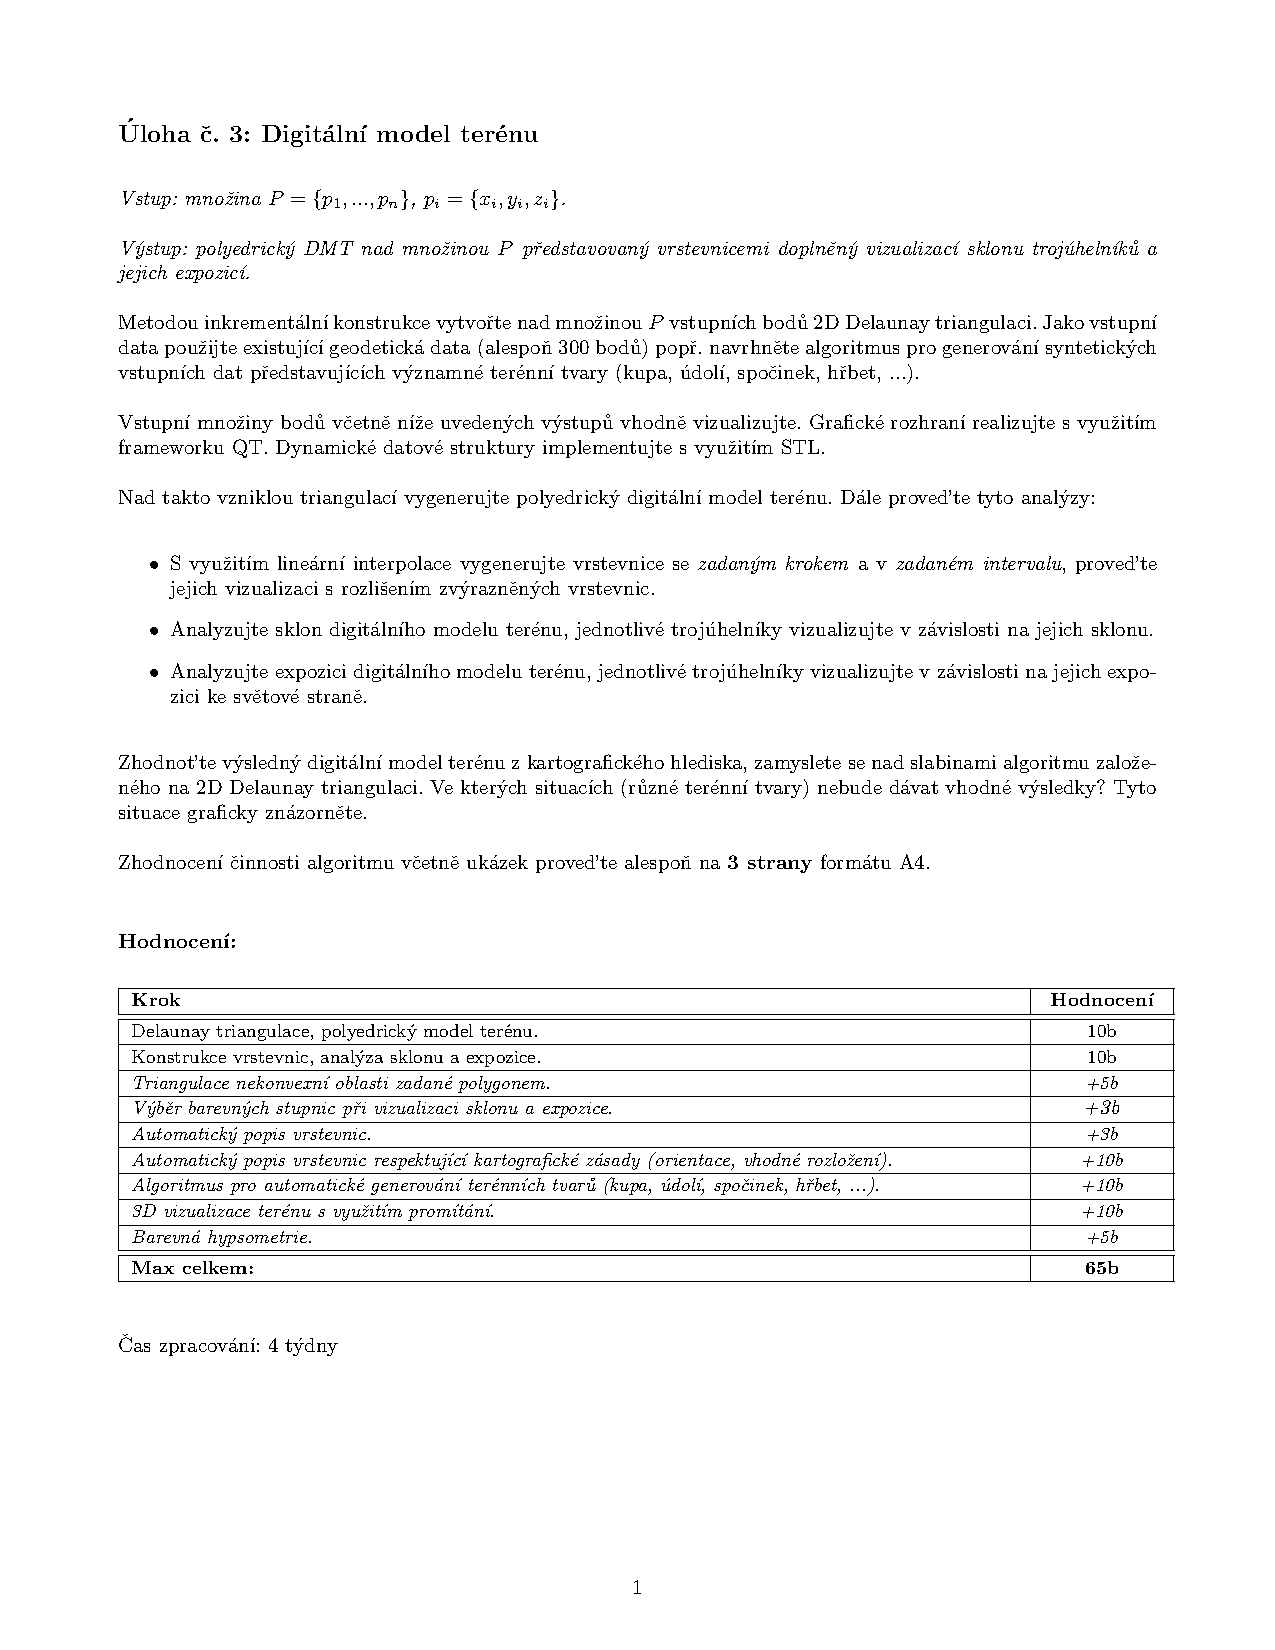
\includepdf{adkcv3}

%---------------------------------------------------------------------
\clearpage
\section{Údaje o bonusových úlohách}




\section{Popis a rozbor problému}




\section{Popisy algoritmů formálním jazykem} \label{popisalg}





\section{Problematické situace a jejich rozbor} \label{problemrozbor}
% (tj. simplexy) + ošetření těchto situací v kódu




\section{Vstupní data}
% formát vstupních dat, popis
Vstupem je textový soubor s~prostorovými souřadnicemi X,Y,Z geodetických bodů. Tyto body jsou považovány za vstupní množinu~P.


\section{Výstupní data}
% formát výstupních dat, popis
Za~výstup je považována grafický výstup vytvořené aplikace. Grafickým výstupem je polyedrický DMT nad množinou~P představovaný vrstevnicemi doplněný vizualizací sklonu trojúhelníků a jejich expozicí. 


\section{Snímky obrazovky vytvořené aplikace a její popis}



\section{Dokumentace}
% popis tříd, datových položek a jednotlivých metod
\subsection{Třída Algorithms}
Tato třída obsahuje výpočetní vzorce pro použité algoritmy.

\textbf{Třída algorithms obsahuje následující veřejné metody:}

\begin{verbatim}
double get2LinesAngle(QPoint &p1, QPoint &p2, QPoint &p3, QPoint &p4)
\end{verbatim}
Metoda vypočte velikost úhlu, který svírají dvě přímky. První přímku tvoří body $p_1, p_2$ a druhou přímku body $p_3, p_4$.\\

\begin{verbatim}
int getPointLinePosition(QPoint &a,QPoint &p1,QPoint &p2)
\end{verbatim}
Metoda určuje, zda~--~li bod leží v~levé či v~pravé polorovině od přímky (hrany polygonu). Vstupními parametry jsou určovaný bod~$a$ a body $p_1, p_2$, které tvoří přímku.\\

\begin{verbatim}
double getPointLineDistance(QPoint &a, QPoint &p1, QPoint &p2)
\end{verbatim}
Metoda určuje vzdálenost bodu~$a$ od přímky tvořenou body $p_1, p_2$.\\

\begin{verbatim}
QPolygon cHullJarvisScan(std::vector <QPoint> &points)
\end{verbatim}
Výpočet konvexní obálky načtených bodů na základě algoritmu Jarvis Scan (kapitola \ref{js}).\\

\begin{verbatim}
std::vector<QPoint> rotate(std::vector<QPoint> &points, double sigma)
\end{verbatim}
Otočení načtených bodů o~zadaný úhel $sigma$.\\

\begin{verbatim}
std::tuple<std::vector<QPoint>, double> minMaxBox(std::vector<QPoint> &points)
\end{verbatim}
Proměnná vracející min~--~max box, tedy vrcholy obdélníka a jeho výměru. Vstupem jsou načtené body.\\

\begin{verbatim}
QPolygon minAreaEnclosingRectangle(std::vector<QPoint> &points)
\end{verbatim}
Určení hlavního směru polygonu s využitím algoritmu Minimum Area Eclosing Rectangle (kapitola \ref{maer}). Na vstupu jsou body polygonu. Výstupem je generalizovaný a pootočený polygon.\\

\begin{verbatim}
QPolygon wallAverage(std::vector<QPoint> &points)
\end{verbatim}
Určení hlavního směru polygonu s využitím algoritmu Wall Average (kapitola \ref{wa}). Na vstupu jsou body polygonu. Výstupem je generalizovaný a pootočený polygon.\\

\begin{verbatim}
double LH(std::vector<QPoint> &points)
\end{verbatim}
Výpočet plochy obecného mnohoúhelníků pomocí LH vzorce.\\ 

\begin{verbatim}
std::vector<QPoint> resizeRectangle(std::vector<QPoint> &points, std::vector<QPoint> &er)
\end{verbatim}
Přepočet velikosti ohraničujícího obdélníku na základě výměry původního polygonu.\\

\begin{verbatim}
QPolygon longestEdge(std::vector<QPoint> &points)
\end{verbatim}
Určení hlavního směru polygonu s využitím algoritmu Longest Edge (kapitola \ref{le}). Na vstupu jsou body polygonu. Výstupem je generalizovaný a pootočený polygon.\\

\begin{verbatim}
QPolygon weightedBisector(std::vector<QPoint> &points)
\end{verbatim}
Určení hlavního směru polygonu s využitím algoritmu Weighted Bisector (kapitola \ref{wb}). Na vstupu jsou body polygonu. Výstupem je generalizovaný a pootočený polygon.\\

\begin{verbatim}
QPolygon cHullQuickHull(std::vector <QPoint> &points)
\end{verbatim}
Výpočet konvexní obálky načtených bodů na základě algoritmu Quick Hull (kapitola \ref{qh}).\\

\begin{verbatim}
void quickHullLocal(int ps, int pe, std::vector<QPoint> &points, QPolygon &ch)
\end{verbatim}
Metoda pro pomocný výpočet rekurentního určení konvexní obálky bodů algoritmem Quick Hull, lokální procedura (kapitola \ref{qh}). Vstupními parametry jsou indexy počátečního a koncového bodu $ps$ a $pe$ vstupní hrany, načtené body a konvexní obálka.\\

    
    
\subsection{Třída Draw}
Tato třída umožňuje vykreslování bodu a polygonů.

\textbf{Třída draw obsahuje následující privátní metody a proměnné:}
\begin{verbatim}
std::vector<QPoint> points
\end{verbatim}
Proměnná se souřadnicemi načtených bodů.\\

\begin{verbatim}
QPolygon ch, er;
\end{verbatim}
Polygony pro ukládání konvexní obálky a ohraničujícího obdélníku.\\

\begin{verbatim}
std::vector<QPolygon> polygons, chs, ers
\end{verbatim}
Proměnná uchovávající pomocné polygony v~průběhu výpočtu a pro vykreslení.\\


\textbf{Třída draw obsahuje následující veřejné metody a proměnné:}
\begin{verbatim}
explicit Draw(QWidget *parent = nullptr)
\end{verbatim}
Prvotní vykreslení bodu mimo okno aplikace.\\

\begin{verbatim}
void paintEvent(QPaintEvent *event)
\end{verbatim}
Metoda, která vykresluje bod či polygony.\\

\begin{verbatim}
void mousePressEvent(QMouseEvent *event)
\end{verbatim}
Metoda určující souřadnice určeného bodu.\\

\begin{verbatim}
void clearAddedData()
\end{verbatim}
Metoda mazající přidaná data z~obrazovky.\\

\begin{verbatim}
void clearDrawing()
\end{verbatim}
Metoda mazající nakreslený polygon z~obrazovky.\\

\begin{verbatim}
std::vector<QPoint> getPoints() {return points;}
\end{verbatim}
Vrací souřadnice lomových bodů polygonu.\\

\begin{verbatim}
std::vector<QPolygon> getPolygons(){return polygons;}
\end{verbatim}
Vrací souřadnice polygonů.\\

\begin{verbatim}
void setCh(QPolygon &ch_) {chs.push_back(ch_);}
\end{verbatim}
Nastavení polygonu konvexní obálky.\\

\begin{verbatim}
void setEr(QPolygon &er_) {ers.push_back(er_);}
\end{verbatim}
Nastavení polygonu ohraničujícího obdélníku.\\

\begin{verbatim}
void clearChs(){chs.clear();}
\end{verbatim}
Smazání polygonu konvexní obálky.\\

\begin{verbatim}
void clearErs(){ers.clear();}
\end{verbatim}
Smazání polygonu ohraničujícího obdélníku.\\

\begin{verbatim}
void drawPolygons(std::vector<QPolygon> &data);
\end{verbatim}
Vykreslení polygonů načtených z~textového souboru.\\

\subsection{Třída Load}
\textbf{Třída draw obsahuje následující veřejnou proměnnou:}
\begin{verbatim}
static std::vector<QPolygon> load_file(std::string &filename)
\end{verbatim}
Umožňuje načítání polygonů z textového souboru.\\

\subsection{Třída SortByX}
\textbf{Třída draw obsahuje následující veřejnou proměnnou:}
\begin{verbatim}
bool operator() (QPoint &p1, QPoint &p2)
\end{verbatim}
Ražení bodů dle jejich x~--~ové souřadnice.\\

\subsection{Třída SortByY}
\textbf{Třída draw obsahuje následující veřejnou proměnnou:}
\begin{verbatim}
bool operator() (QPoint &p1, QPoint &p2)
\end{verbatim}
Ražení bodů dle jejich y~--~ové souřadnice.\\

\subsection{Třída Widget}
Tato třída propojuje uživatelské rozhraní aplikace s kódem. Je vytvořena v sekci \emph{Design}.

\textbf{Třída widget obsahuje následující privátní metody a proměnné:}
\begin{verbatim}
void on_pushButtonClear_clicked()
\end{verbatim}
Vymazání kresby. Propojení s~tlačítkem \emph{Clear drawing}.\\

\begin{verbatim}
void on_pushButtonLoad_clicked()
\end{verbatim}
Načtení lomových bodů polygonů z~textového souboru. Propojení s~tlačítkem \emph{Load file with polygon}.\\

\begin{verbatim}
void on_pushButton_clicked()
\end{verbatim}
Spuštění funkce Building Simplify s~vybraným algoritmem. Propojení s~tlačítkem \emph{Building Simplify}.\\

\begin{verbatim}
void on_pushButtonClearData_clicked()
\end{verbatim}
Vymazání přidaných dat. Propojení s~tlačítkem \emph{Clear added data}.\\

\begin{verbatim}
void processPoints(std::vector<QPoint> &points)
\end{verbatim}
Volba použitého algoritmu na základě výběru z~combo boxů.\\



\section{Závěr}






\subsection{Možné či neřešené problémy} \label{mcn_problemy}


\subsection{Náměty na vylepšení} \label{vylepseni}



\begin{flushright}
V Praze 30.11.2021\\
\vspace{2mm}
Bc. Pane Kuzmanov\\
Bc. František Mužík\\
\end{flushright}


%---------------------------------------------------------------------
\clearpage 
\section*{Použitá literatura}
\renewcommand{\section}[2]{}%
\bibliographystyle{acm}
\bibliography{Literatura_u2_adk}


\end{document}
